\section{Structure}
\subsection{Introduction}

\href{https://learn.microsoft.com/en-us/windows/win32/debug/pe-format}{PE Format} official documentation describe default values 

\href{https://www.openrce.org/reference_library/files/reference/PE%20Format.pdf}{Open RCE - PE Format}

\begin{figure}[!ht]
    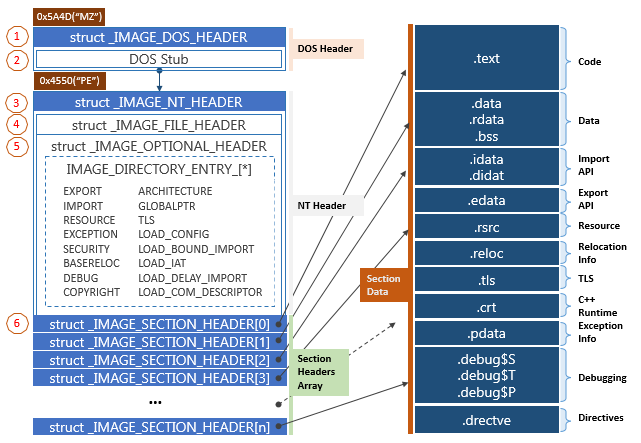
\includegraphics[width=\linewidth]{knowledge/pe/images/Gen_DD_Win_PE_Format.png}
    \caption{PE overview}
    \label{fig:pe_overview}
\end{figure}

\begin{figure}[!ht]
    \includegraphics[width=\linewidth]{knowledge/pe/images/pe-format.pdf}
    \caption{PE Details}
    \label{fig:pe_details}
\end{figure}

All structures are defined in \href{https://learn.microsoft.com/fr-fr/windows/win32/api/winnt/}{winnt.h}

\subsection{Relative Virtual Address}
An RVA specifies the offset of an element (like a function, data structure, or section) from the base address where the PE file is loaded into memory.

When a PE file is loaded into memory, the operating system assigns it a {\bf base address}. This is the starting point in virtual memory where the entire image of the PE file is mapped.

Mathematically: \verb+RVA=Virtual Address - Base Address+

Absolute Virtual Address is the \verb-RVA + Base Address-

RVAs are heavily used in the PE file's import and export tables to specify the locations of functions and data. For example, the addresses of imported functions are given as RVAs, which are resolved to actual virtual addresses at runtime.

RVAs are crucial for relocating a PE file when it cannot be loaded at its preferred base address. The loader adjusts all RVAs accordingly.

the PE file sections are aligned differently in memory compared to how they are laid out on disk, the RVA does not directly correspond to an offset in the file. 

To convert an RVA to a file offset (or vice versa), you need to:
\begin{itemize}
    \item Identify the section in which the RVA falls.
    \item Use the section's information (like \verb+PointerToRawData+ and \verb+VirtualAddress+) to compute the corresponding file offset.
\end{itemize}


\subsection{DOS}

\subsubsection{DOS Header}
The DOS header (also called the MS-DOS header) is a 64-byte-long structure that exists at the start of the PE file.

It’s there because of backward compatibility reasons. 

This header makes the file an MS-DOS executable, so when it’s loaded on MS-DOS the DOS stub gets executed instead of the actual program.
Without this header, if you attempt to load the executable on MS-DOS it will not be loaded and will just produce a generic error.

\begin{verbatim}
typedef struct _IMAGE_DOS_HEADER {      // DOS .EXE header
  WORD   e_magic;                     // Magic number
  WORD   e_cblp;                      // Bytes on last page of file
  WORD   e_cp;                        // Pages in file
  WORD   e_crlc;                      // Relocations
  WORD   e_cparhdr;                   // Size of header in paragraphs
  WORD   e_minalloc;                  // Minimum extra paragraphs needed
  WORD   e_maxalloc;                  // Maximum extra paragraphs needed
  WORD   e_ss;                        // Initial (relative) SS value
  WORD   e_sp;                        // Initial SP value
  WORD   e_csum;                      // Checksum
  WORD   e_ip;                        // Initial IP value
  WORD   e_cs;                        // Initial (relative) CS value
  WORD   e_lfarlc;                    // File address of relocation table
  WORD   e_ovno;                      // Overlay number
  WORD   e_res[4];                    // Reserved words
  WORD   e_oemid;                     // OEM identifier (for e_oeminfo)
  WORD   e_oeminfo;                   // OEM information; e_oemid specific
  WORD   e_res2[10];                  // Reserved words
  LONG   e_lfanew;                    // File address of new exe header
} IMAGE_DOS_HEADER, *PIMAGE_DOS_HEADER;
\end{verbatim}

\begin{itemize}

    \item \verb+e_magic+: This is the first member of the DOS Header, it’s a \verb+WORD+ (2 bytes), it’s usually called the magic number. It has a fixed value of \verb+0x5A4D+ or \verb+MZ+ in ASCII, and it serves as a signature that marks the file as an MS-DOS executable.
    \item \verb+e_lfanew+: This is the last member of the DOS header structure, it’s located at offset \verb+0x3C+ into the DOS header and it holds an offset to the start of the NT headers. This member is important to the PE loader on Windows systems because it tells the loader where to look for the file header.
\end{itemize}

\subsubsection{DOS stub}

The DOS stub is an MS-DOS program that prints an error message saying that the executable is not compatible with DOS then exits. 

This is what gets executed when the program is loaded in MS-DOS, the default error message is “This program cannot be run in DOS mode.”, however this message can be changed by the user during compile time.



\subsection{Rich Header}

Chunk of data we haven’t talked about lying between the DOS Stub and the start of the NT Headers.

The \href{https://github.com/RichHeaderResearch/RichPE}{Rich header} is an undocumented header contained within PE files compiled and linked using the Microsoft Visual Studio toolset. It contains information about the build environment that the PE file was created in.

See also \href{https://0xrick.github.io/win-internals/pe3/#rich-header}{Rich Header}

\subsection{NT Headers}

\begin{verbatim}
typedef struct _IMAGE_NT_HEADERS {
    DWORD                 Signature; // PE\0\0 or 0x00004550
    IMAGE_FILE_HEADER     FileHeader;
    IMAGE_OPTIONAL_HEADER OptionalHeader;
} IMAGE_NT_HEADERS, *PIMAGE_NT_HEADERS;

typedef struct _IMAGE_NT_HEADERS64 {
    DWORD Signature;
    IMAGE_FILE_HEADER FileHeader;
    IMAGE_OPTIONAL_HEADER64 OptionalHeader;
} IMAGE_NT_HEADERS64, *PIMAGE_NT_HEADERS64;
\end{verbatim}

\subsubsection{File Header}
Also called {\emph The COFF File Header}, the File Header is a structure that holds some information about the PE file.
\begin{verbatim}
typedef struct _IMAGE_FILE_HEADER {
    WORD  Machine;              // machine type used for compilation
    WORD  NumberOfSections; 
    DWORD TimeDateStamp;        // of the file creation  
    DWORD PointerToSymbolTable;
    DWORD NumberOfSymbols;
    WORD  SizeOfOptionalHeader;
    WORD  Characteristics;
} IMAGE_FILE_HEADER, *PIMAGE_FILE_HEADER;
\end{verbatim}

\begin{itemize}

    \item \verb+Machine+: This is a number that indicates the type of machine (CPU Architecture) the executable is targeting, this field can have a lot of values.For a complete list of possible values you can check the \href{https://learn.microsoft.com/en-us/windows/win32/debug/pe-format#machine-types}{official Microsoft documentation}.
    \item \verb+NumberOfSections+: This field holds the number of sections (or the number of section headers aka. the size of the section table.).
    \item \verb+TimeDateStamp+: A unix timestamp that indicates when the file was created.
    \item \verb+PointerToSymbolTable+ and NumberOfSymbols: These two fields hold the file offset to the COFF symbol table and the number of entries in that symbol table, however they get set to 0 which means that no COFF symbol table is present, this is done because the COFF debugging information is deprecated.
    \item \verb+SizeOfOptionalHeader+: The size of the Optional Header.
    \item \verb+Characteristics+: A flag that indicates the attributes of the file, these attributes can be things like the file being executable, the file being a system file and not a user program, and a lot of other things. A complete list of these flags can be found on the \href{https://learn.microsoft.com/en-us/windows/win32/debug/pe-format#characteristics}{official Microsoft documentation}.

\end{itemize}


\subsubsection{Optional Header}
The most important header of the NT headers, the PE loader looks for specific information provided by that header to be able to load and run the executable.

It’s called the optional header because some file types like object files don’t have it, however this header is essential for image files. 

\begin{verbatim}
    typedef struct _IMAGE_OPTIONAL_HEADER {
        WORD                 Magic;
        BYTE                 MajorLinkerVersion;
        BYTE                 MinorLinkerVersion;
        DWORD                SizeOfCode;
        DWORD                SizeOfInitializedData;
        DWORD                SizeOfUninitializedData;
        DWORD                AddressOfEntryPoint;
        DWORD                BaseOfCode;
        DWORD                BaseOfData;
        DWORD                ImageBase;
        DWORD                SectionAlignment;
        DWORD                FileAlignment;
        WORD                 MajorOperatingSystemVersion;
        WORD                 MinorOperatingSystemVersion;
        WORD                 MajorImageVersion;
        WORD                 MinorImageVersion;
        WORD                 MajorSubsystemVersion;
        WORD                 MinorSubsystemVersion;
        DWORD                Win32VersionValue;
        DWORD                SizeOfImage;
        DWORD                SizeOfHeaders;
        DWORD                CheckSum;
        WORD                 Subsystem;
        WORD                 DllCharacteristics;
        DWORD                SizeOfStackReserve;
        DWORD                SizeOfStackCommit;
        DWORD                SizeOfHeapReserve;
        DWORD                SizeOfHeapCommit;
        DWORD                LoaderFlags;
        DWORD                NumberOfRvaAndSizes;
        IMAGE_DATA_DIRECTORY DataDirectory[IMAGE_NUMBEROF_DIRECTORY_ENTRIES];
      } IMAGE_OPTIONAL_HEADER32, *PIMAGE_OPTIONAL_HEADER32;
\end{verbatim}

It doesn’t have a fixed size, that’s why the \verb+IMAGE_FILE_HEADER.SizeOfOptionalHeader+ member exists.

\begin{itemize}

    \item \verb+MMagic+:integer that identifies the state of the image, the documentation mentions three common values:
        \begin{itemize}

            \item \verb+0x10B+: Identifies the image as a PE32 executable.
            \item \verb+0x20B+: Identifies the image as a PE32+ executable.
            \item \verb+0x107+: Identifies the image as a ROM image.
        \end{itemize}
    The value of this field is what determines whether the executable is 32-bit or 64-bit, \verb+IMAGE_FILE_HEADER.Machine+ is ignored by the Windows PE loader.
    \item \verb+MajorLinkerVersion+ and \verb+MinorLinkerVersion+: The linker major and minor version numbers.
    \item \verb+SizeOfCode+: size of the code (\verb+.text+) section, or the sum of all code sections if there are multiple sections.
    \item \verb+SizeOfInitializedData+: size of the initialized data (\verb+.data+) section, or the sum of all initialized data sections if there are multiple sections.
    \item \verb+SizeOfUninitializedData+: size of the uninitialized data (\verb+.bss+) section, or the sum of all uninitialized data sections if there are multiple sections.
    \item \verb+AddressOfEntryPoint+: An RVA of the entry point when the file is loaded into memory. The documentation states that for program images this relative address points to the starting address and for device drivers it points to initialization function. For DLLs an entry point is optional, and in the case of entry point absence the \verb+AddressOfEntryPoint+ field is set to 0.
    \item \verb+BaseOfCode+: An RVA of the start of the code section when the file is loaded into memory.
    \item \verb+BaseOfData+ (PE32 Only): An RVA of the start of the data section when the file is loaded into memory.
    \item \verb+ImageBase+: This field holds the preferred address of the first byte of image when loaded into memory (the preferred base address), this value must be a multiple of 64K. Due to memory protections like ASLR, and a lot of other reasons, the address specified by this field is almost never used, in this case the PE loader chooses an unused memory range to load the image into, after loading the image into that address the loader goes into a process called the {\bf relocating} where it fixes the constant addresses within the image to work with the new image base, there’s a special section that holds information about places that will need fixing if relocation is needed, that section is called the relocation section (.reloc), more on that in the upcoming posts.
    \item \verb+SectionAlignment+: value that gets used for section alignment in memory (in bytes), sections are aligned in memory boundaries that are multiples of this value. The documentation states that this value defaults to the page size for the architecture and it can’t be less than the value of \verb+FileAlignment+.
    \item \verb+FileAlignment+: Similar to \verb+SectionAligment+ value that gets used for section raw data alignment on disk (in bytes), if the size of the actual data in a section is less than the \verb+FileAlignment+ value, the rest of the chunk gets padded with zeroes to keep the alignment boundaries. The documentation states that this value should be a power of 2 between 512 and 64K, and if the value of \verb+SectionAlignment+ is less than the architecture’s page size then the sizes of \verb+FileAlignment+ and \verb+SectionAlignment+ must match.
    \item \verb+MajorOperatingSystemVersion+, \verb+MinorOperatingSystemVersion+, \verb+MajorImageVersion+, \verb+MinorImageVersion+, \verb+MajorSubsystemVersion+ and \verb+MinorSubsystemVersion+: These members of the structure specify the major version number of the required operating system, the minor version number of the required operating system, the major version number of the image, the minor version number of the image, the major version number of the subsystem and the minor version number of the subsystem respectively.
    \item \verb+Win32VersionValue+: A reserved field that the documentation says should be set to 0.
    \item \verb+SizeOfImage+: The size of the image file (in bytes), including all headers. It gets rounded up to a multiple of \verb+SectionAlignment+ because this value is used when loading the image into memory.
    \item \verb+SizeOfHeaders+: The combined size of the DOS stub, PE header (NT Headers), and section headers rounded up to a multiple of \verb+FileAlignment+.
    \item \verb+CheckSum+: A checksum of the image file, it’s used to validate the image at load time.
    \item \verb+Subsystem+: This field specifies the Windows subsystem (if any) that is required to run the image, A complete list of the possible values of this field can be found on the \href{https://learn.microsoft.com/en-us/windows/win32/debug/pe-format#windows-subsystem}{official Microsoft documentation}.
    \item \verb+DLLCharacteristics+: This field defines some characteristics of the executable image file, like if it’s NX compatible and if it can be relocated at run time. I have no idea why it’s named DLLCharacteristics, it exists within normal executable image files and it defines characteristics that can apply to normal executable files. A complete list of the possible flags for DLLCharacteristics can be found on the \href{https://learn.microsoft.com/en-us/windows/win32/debug/pe-format#windows-subsystem}{official Microsoft documentation}.
    \item \verb+SizeOfStackReserve+, \verb+SizeOfStackCommit+, \verb+SizeOfHeapReserve+ and \verb+SizeOfHeapCommit+: These fields specify the size of the stack to reserve, the size of the stack to commit, the size of the local heap space to reserve and the size of the local heap space to commit respectively.
    \item \verb+LoaderFlags+: A reserved field that the documentation says should be set to 0.
    \item \verb+NumberOfRvaAndSizes+ : Size of the \verb+DataDirectory+ array.
    \item \verb+DataDirectory+: An array of \verb+IMAGE_DATA_DIRECTORY+ structures.
\end{itemize}

\subsubsection{Data Directories}
\begin{verbatim}
IMAGE_DATA_DIRECTORY DataDirectory[IMAGE_NUMBEROF_DIRECTORY_ENTRIES];
#define IMAGE_NUMBEROF_DIRECTORY_ENTRIES    16
\end{verbatim}

\begin{verbatim}
#define IMAGE_DIRECTORY_ENTRY_EXPORT          0   // Export Directory
#define IMAGE_DIRECTORY_ENTRY_IMPORT          1   // Import Directory
#define IMAGE_DIRECTORY_ENTRY_RESOURCE        2   // Resource Directory
#define IMAGE_DIRECTORY_ENTRY_EXCEPTION       3   // Exception Directory
#define IMAGE_DIRECTORY_ENTRY_SECURITY        4   // Security Directory
#define IMAGE_DIRECTORY_ENTRY_BASERELOC       5   // Base Relocation Table
#define IMAGE_DIRECTORY_ENTRY_DEBUG           6   // Debug Directory
//      IMAGE_DIRECTORY_ENTRY_COPYRIGHT       7   // (X86 usage)
#define IMAGE_DIRECTORY_ENTRY_ARCHITECTURE    7   // Architecture Specific Data
#define IMAGE_DIRECTORY_ENTRY_GLOBALPTR       8   // RVA of GP
#define IMAGE_DIRECTORY_ENTRY_TLS             9   // TLS Directory
#define IMAGE_DIRECTORY_ENTRY_LOAD_CONFIG    10   // Load Configuration Directory
#define IMAGE_DIRECTORY_ENTRY_BOUND_IMPORT   11   // Bound Import Directory in headers
#define IMAGE_DIRECTORY_ENTRY_IAT            12   // Import Address Table
#define IMAGE_DIRECTORY_ENTRY_DELAY_IMPORT   13   // Delay Load Import Descriptors
#define IMAGE_DIRECTORY_ENTRY_COM_DESCRIPTOR 14   // COM Runtime descriptor
\end{verbatim}

\begin{verbatim}
    typedef struct _IMAGE_DATA_DIRECTORY {
        DWORD   VirtualAddress;
        DWORD   Size;
    } IMAGE_DATA_DIRECTORY, *PIMAGE_DATA_DIRECTORY;    
\end{verbatim}

It’s a very simple structure with only two members, first one being an RVA pointing to the start of the Data Directory and the second one being the size of the Data Directory.


Basically a Data Directory is a piece of data located within one of the sections of the PE file. Data Directories contain useful information needed by the loader

\subsection{Section Headers}


These headers contain information about the sections of the PE file. The size of the Section Headers is \verb+_IMAGE_FILE_HEADER.NumberOfSections+

It’s an array of \verb+IMAGE_SECTION_HEADER+ structures, each of which describes a single section, denoting its size in the file and in memory (\verb+SizeOfRawData+ and \verb+VirtualSize+), its file offset and virtual address (\verb+PointerToRawData+ and \verb+VirtualAddress+), relocation information, and any flags (\verb+Characteristics+).

\begin{verbatim}
    typedef struct _IMAGE_SECTION_HEADER {
        BYTE    Name[IMAGE_SIZEOF_SHORT_NAME];
        union {
                DWORD   PhysicalAddress;
                DWORD   VirtualSize;
        } Misc;
        DWORD   VirtualAddress;
        DWORD   SizeOfRawData;
        DWORD   PointerToRawData;
        DWORD   PointerToRelocations;
        DWORD   PointerToLinenumbers;
        WORD    NumberOfRelocations;
        WORD    NumberOfLinenumbers;
        DWORD   Characteristics;
    } IMAGE_SECTION_HEADER, *PIMAGE_SECTION_HEADER;    
\end{verbatim}
\begin{itemize}

        \item \verb+Name+: First field of the Section Header, a byte array of the size \verb+IMAGE_SIZEOF_SHORT_NAME+ that holds the name of the section. \verb+IMAGE_SIZEOF_SHORT_NAME+ has the value of 8 meaning that a section name can’t be longer than 8 characters. For longer names the official documentation mentions a work-around by filling this field with an offset in the string table, however executable images do not use a string table so this limitation of 8 characters holds for executable images.
        \item \verb+PhysicalAddress+ or \verb+VirtualSize+: A union defines multiple names for the same thing, this field contains the total size of the section when it’s loaded in memory.
        \item \verb+VirtualAddress+: The documentation states that for executable images this field holds the address of the first byte of the section relative to the image base when loaded in memory, and for object files it holds the address of the first byte of the section before relocation is applied.
        \item \verb+SizeOfRawData+: This field contains the size of the section on disk, it must be a multiple of \verb+IMAGE_OPTIONAL_HEADER.FileAlignment+. \verb+SizeOfRawData+ and \verb+VirtualSize+ can be different.
        \item \verb+PointerToRawData+: A pointer to the first page of the section within the file, for executable images it must be a multiple of \verb+IMAGE_OPTIONAL_HEADER.FileAlignment+.
        \item \verb+PointerToRelocations+: A file pointer to the beginning of relocation entries for the section. It’s set to 0 for executable files.
        \item \verb+PointerToLineNumbers+: A file pointer to the beginning of COFF line-number entries for the section. It’s set to 0 because COFF debugging information is deprecated.
        \item \verb+NumberOfRelocations+: The number of relocation entries for the section, it’s set to 0 for executable images.
        \item \verb+NumberOfLinenumbers+: The number of COFF line-number entries for the section, it’s set to 0 because COFF debugging information is deprecated.
        \item \verb+Characteristics+: Flags that describe the characteristics of the section.  These characteristics are things like if the section contains executable code, contains initialized/uninitialized data, can be shared in memory. A complete list of section characteristics flags can be found on the \href{https://learn.microsoft.com/en-us/windows/win32/debug/pe-format#section-flags}{official Microsoft documentation}.

\end{itemize}

\subsection{Sections}

Sections are the containers of the actual data of the executable file, they occupy the rest of the PE file.

Some sections have special names that indicate their purpose, we’ll go over some of them, and a full list of these names can be found on the \href{Some sections have special names that indicate their purpose, we’ll go over some of them, and a full list of these names can be found on the official Microsoft documentation }{official Microsoft documentation}.


